\documentclass[../../main.tex]{subfiles}

\begin{document}

\section{Overview}

In this section, the entities defined in the class diagram and their relationships are formally analyzed using the Alloy declarative specification language. 
Each relevant entity is included in the Alloy model and its relationships are tested for consistency. The focus of the model is to describe how Telengana's policy makers and Agronomists help farmers with production improvement. Different worlds were generated to highlight specific aspects of the model.

\section{Alloy model}

\subsection{Source code}

\begin{lstlisting}[language=alloy]
open util/integer

/*********************** PRIMITIVE TYPES ************************/

sig Username, Password, id, personalinformation{}

/************************* SIGNATURES ***************************/

abstract sig User {
	ID: id,
	username: Username,
	password: Password,
	PersonalInformation: personalinformation
}

sig PolicyMaker extends User {
	publish: some Policy
}
sig Farmer extends User {
	create: some DiscussionForum,
	join: some DiscussionForum,
	suggest: some Suggestion, 
}
sig Agronomist extends User {
	responsibilityArea: one Area, 
	suggest: some Suggestion, 
	schedule: one DailyPlan
}

sig Area {
	farms: some Farm
}

sig Farm {
	farmers: one Farmer
}

sig  DiscussionForum{
} {
}

sig Policy {
}

sig DailyPlan {
	receiver:  one Agronomist
}

sig Suggestion {
	give: some Farmer
}

/************************** FACTS *******************************/

// Usernames of registered users are unique.
fact uniqueUsernames {
	no disjoint u1, u2: User |
		u1.username = u2.username
}


// A farm is always belonging to a area
fact farmAlwaysInArea {
all f: Farm | one a: Area | f in a.farms
}
//A farmer is always belonging to a farm
fact farmerAlwaysInFarm {
all f: Farmer | one a: Farm | f in a.farmers
}
// A daily plan is always belonging to a agronomist
fact dailyPlanAlwaysInAgronomist {
all d: DailyPlan | one a: Agronomist | d in a.schedule
}

// A area is always associated with only one agronomist
fact areaAlwaysAssociated
{
all a: Area | one g: Agronomist | a in g.responsibilityArea
}

// A suggestion is always associated with only one agronomist
fact suggestionAlwaysAssociated
{
all s: Suggestion | one a: Agronomist | s in a.suggest
}

// A policy is always belonging to a policy maker
fact policyAlwaysInpolicyMaker {
all p: Policy | one m: PolicyMaker | p in m.publish
}


/************************ PREDICATES ****************************/

pred show { 
	#PolicyMaker = 2
	#Farmer >= 10
	#Agronomist = 5
	#Suggestion = 10
	#Farm >= 10 
	#Policy = 1
	#Area = 6
}
/************************** WORLDS ******************************/
run show for 50
  
\end{lstlisting}

\subsection{Predicates execution and assertions checks}

\begin{figure}[H]
  \centering
  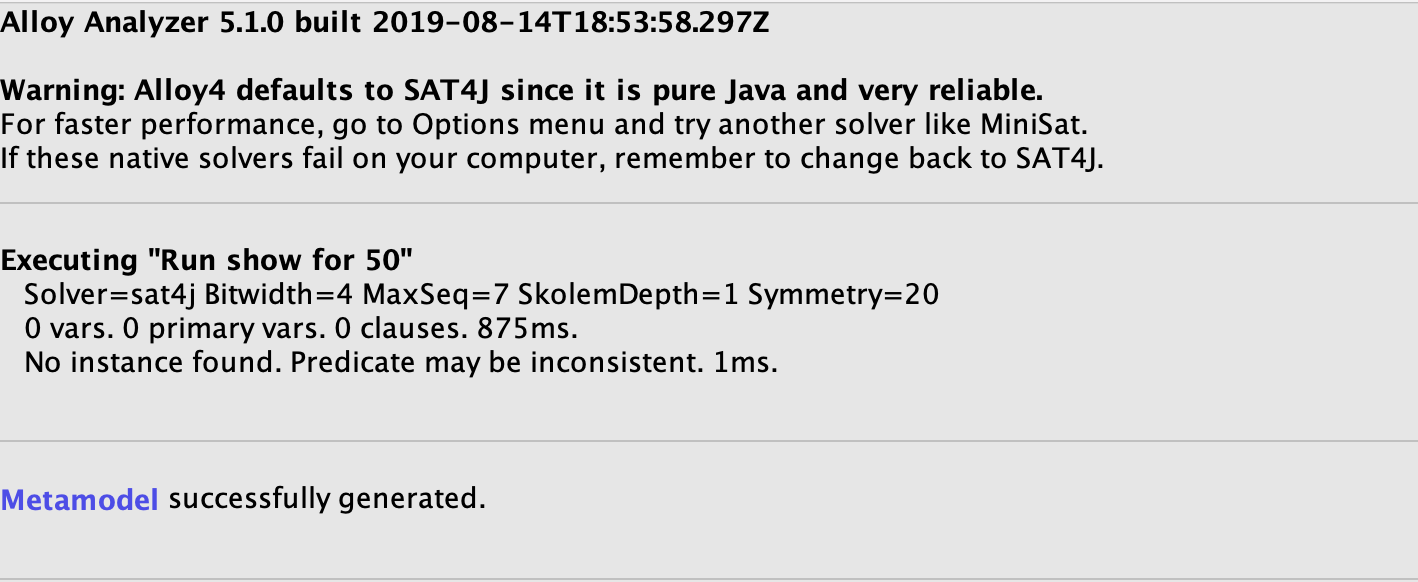
\includegraphics[width=\textwidth]{RASD/image/redicates_execution_and assertions_checks.jpg}
  \caption{Results of the execution of the Alloy predicates and assertions checks}
\end{figure}

\subsection{Resulting worlds}

\begin{figure}[H]
  \centering
  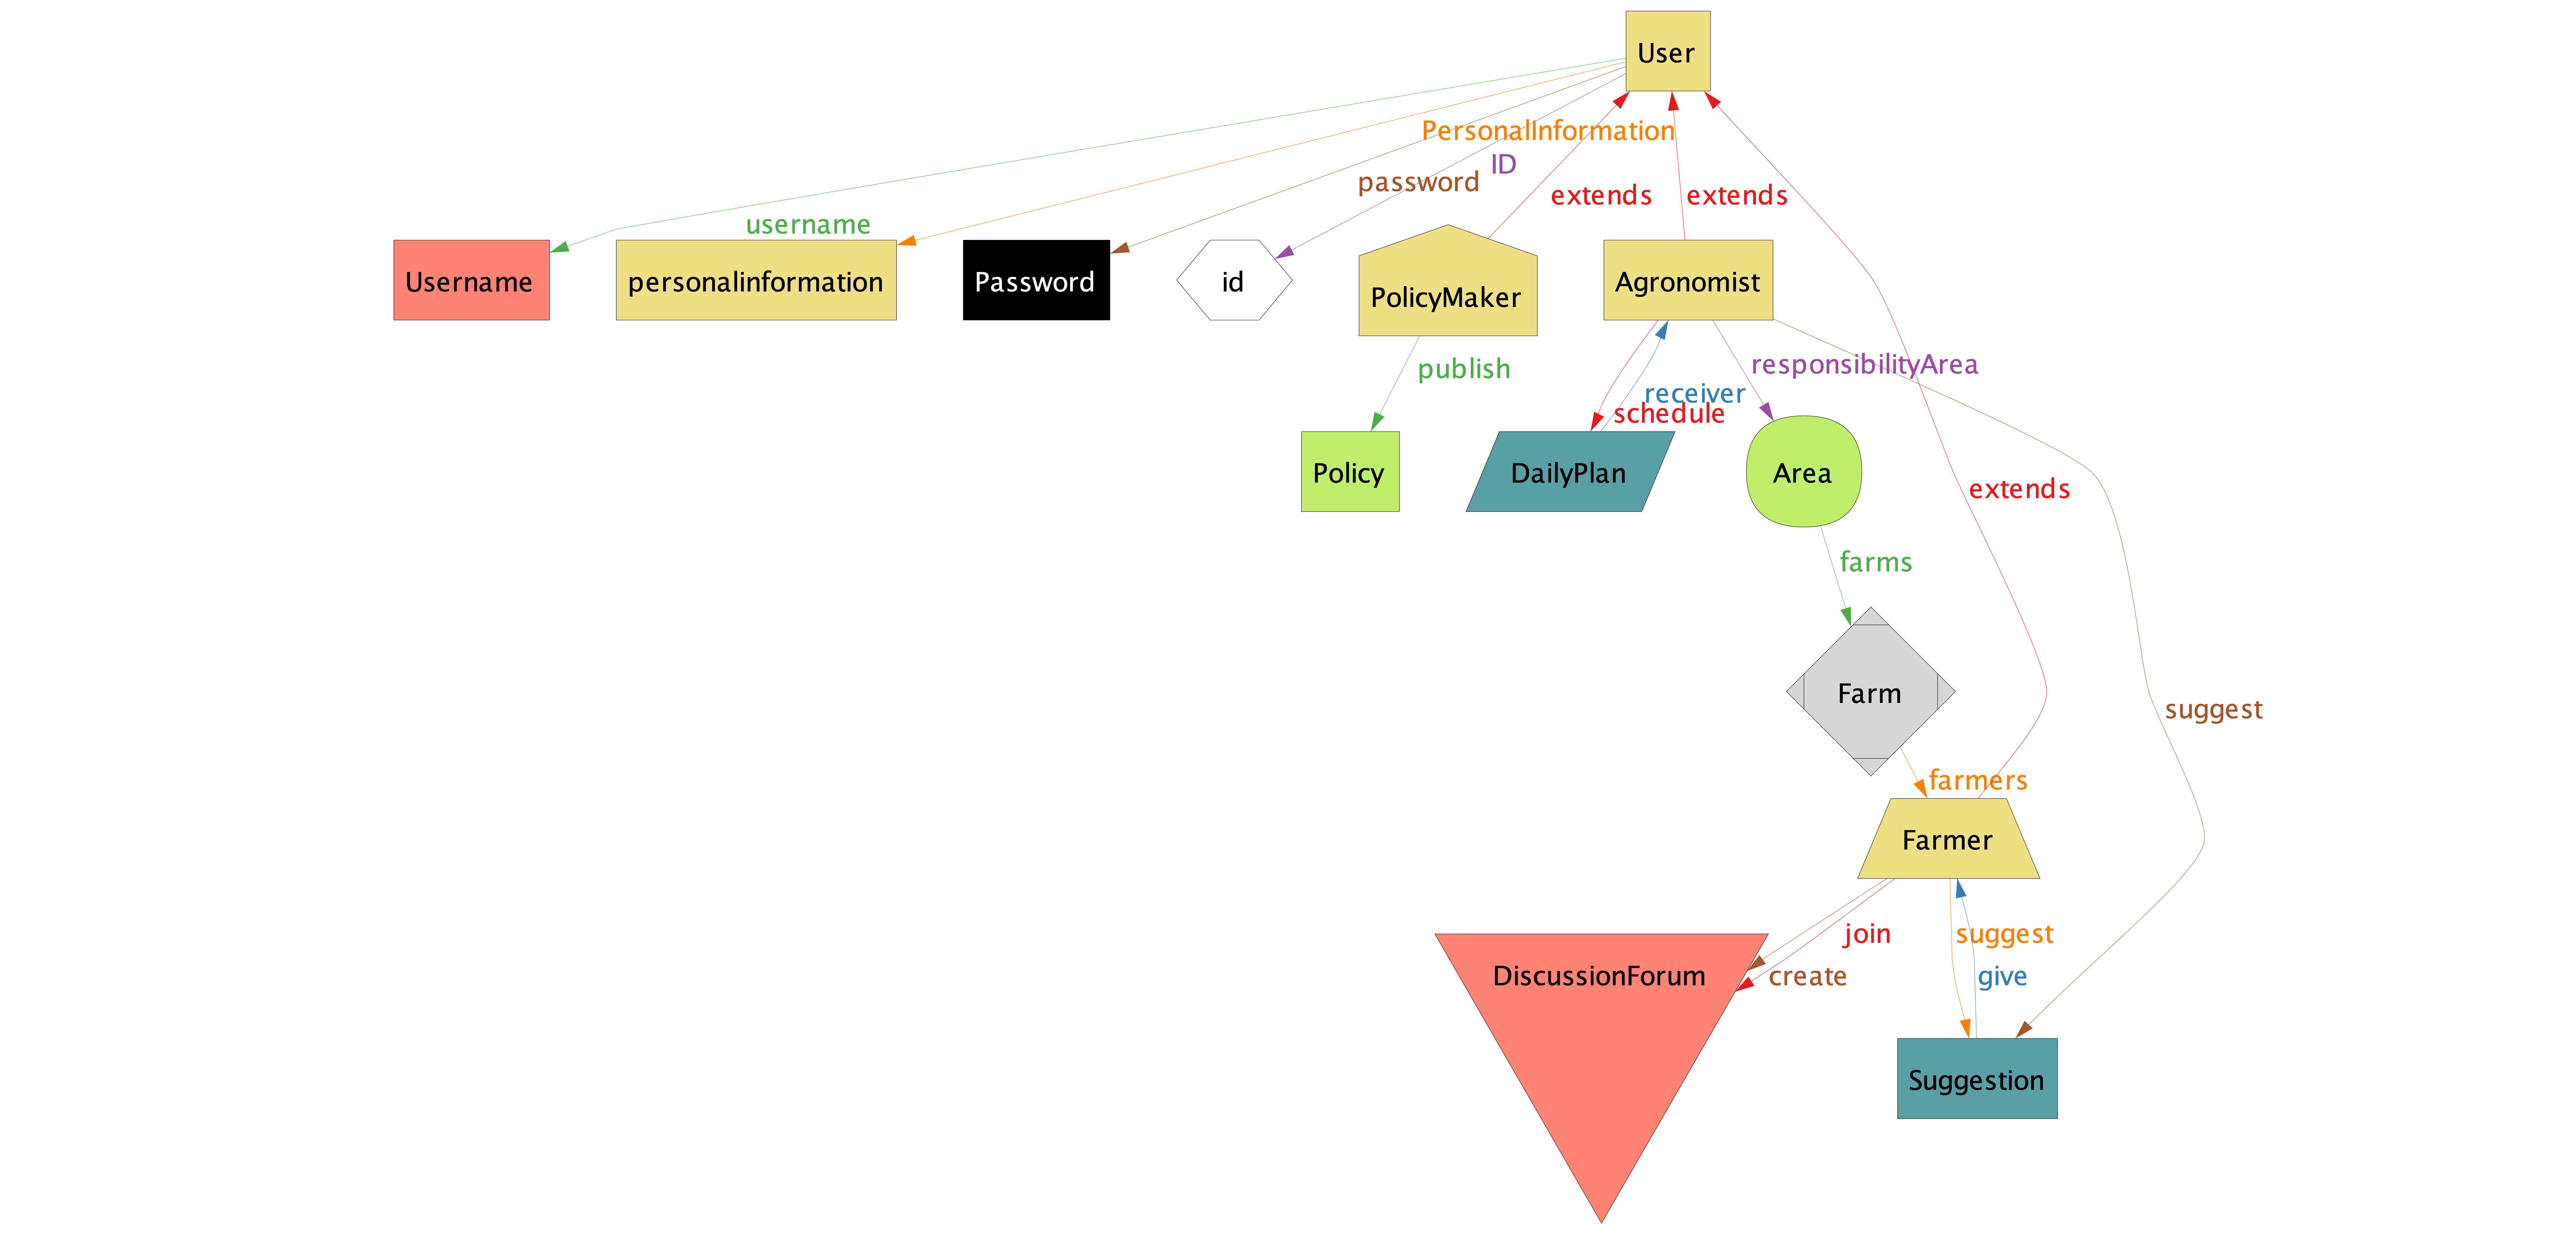
\includegraphics[width=\textwidth]{RASD/image/Alloy.png}
  \caption{One of the worlds generated}
\end{figure}

\begin{figure}[H]
  \centering
  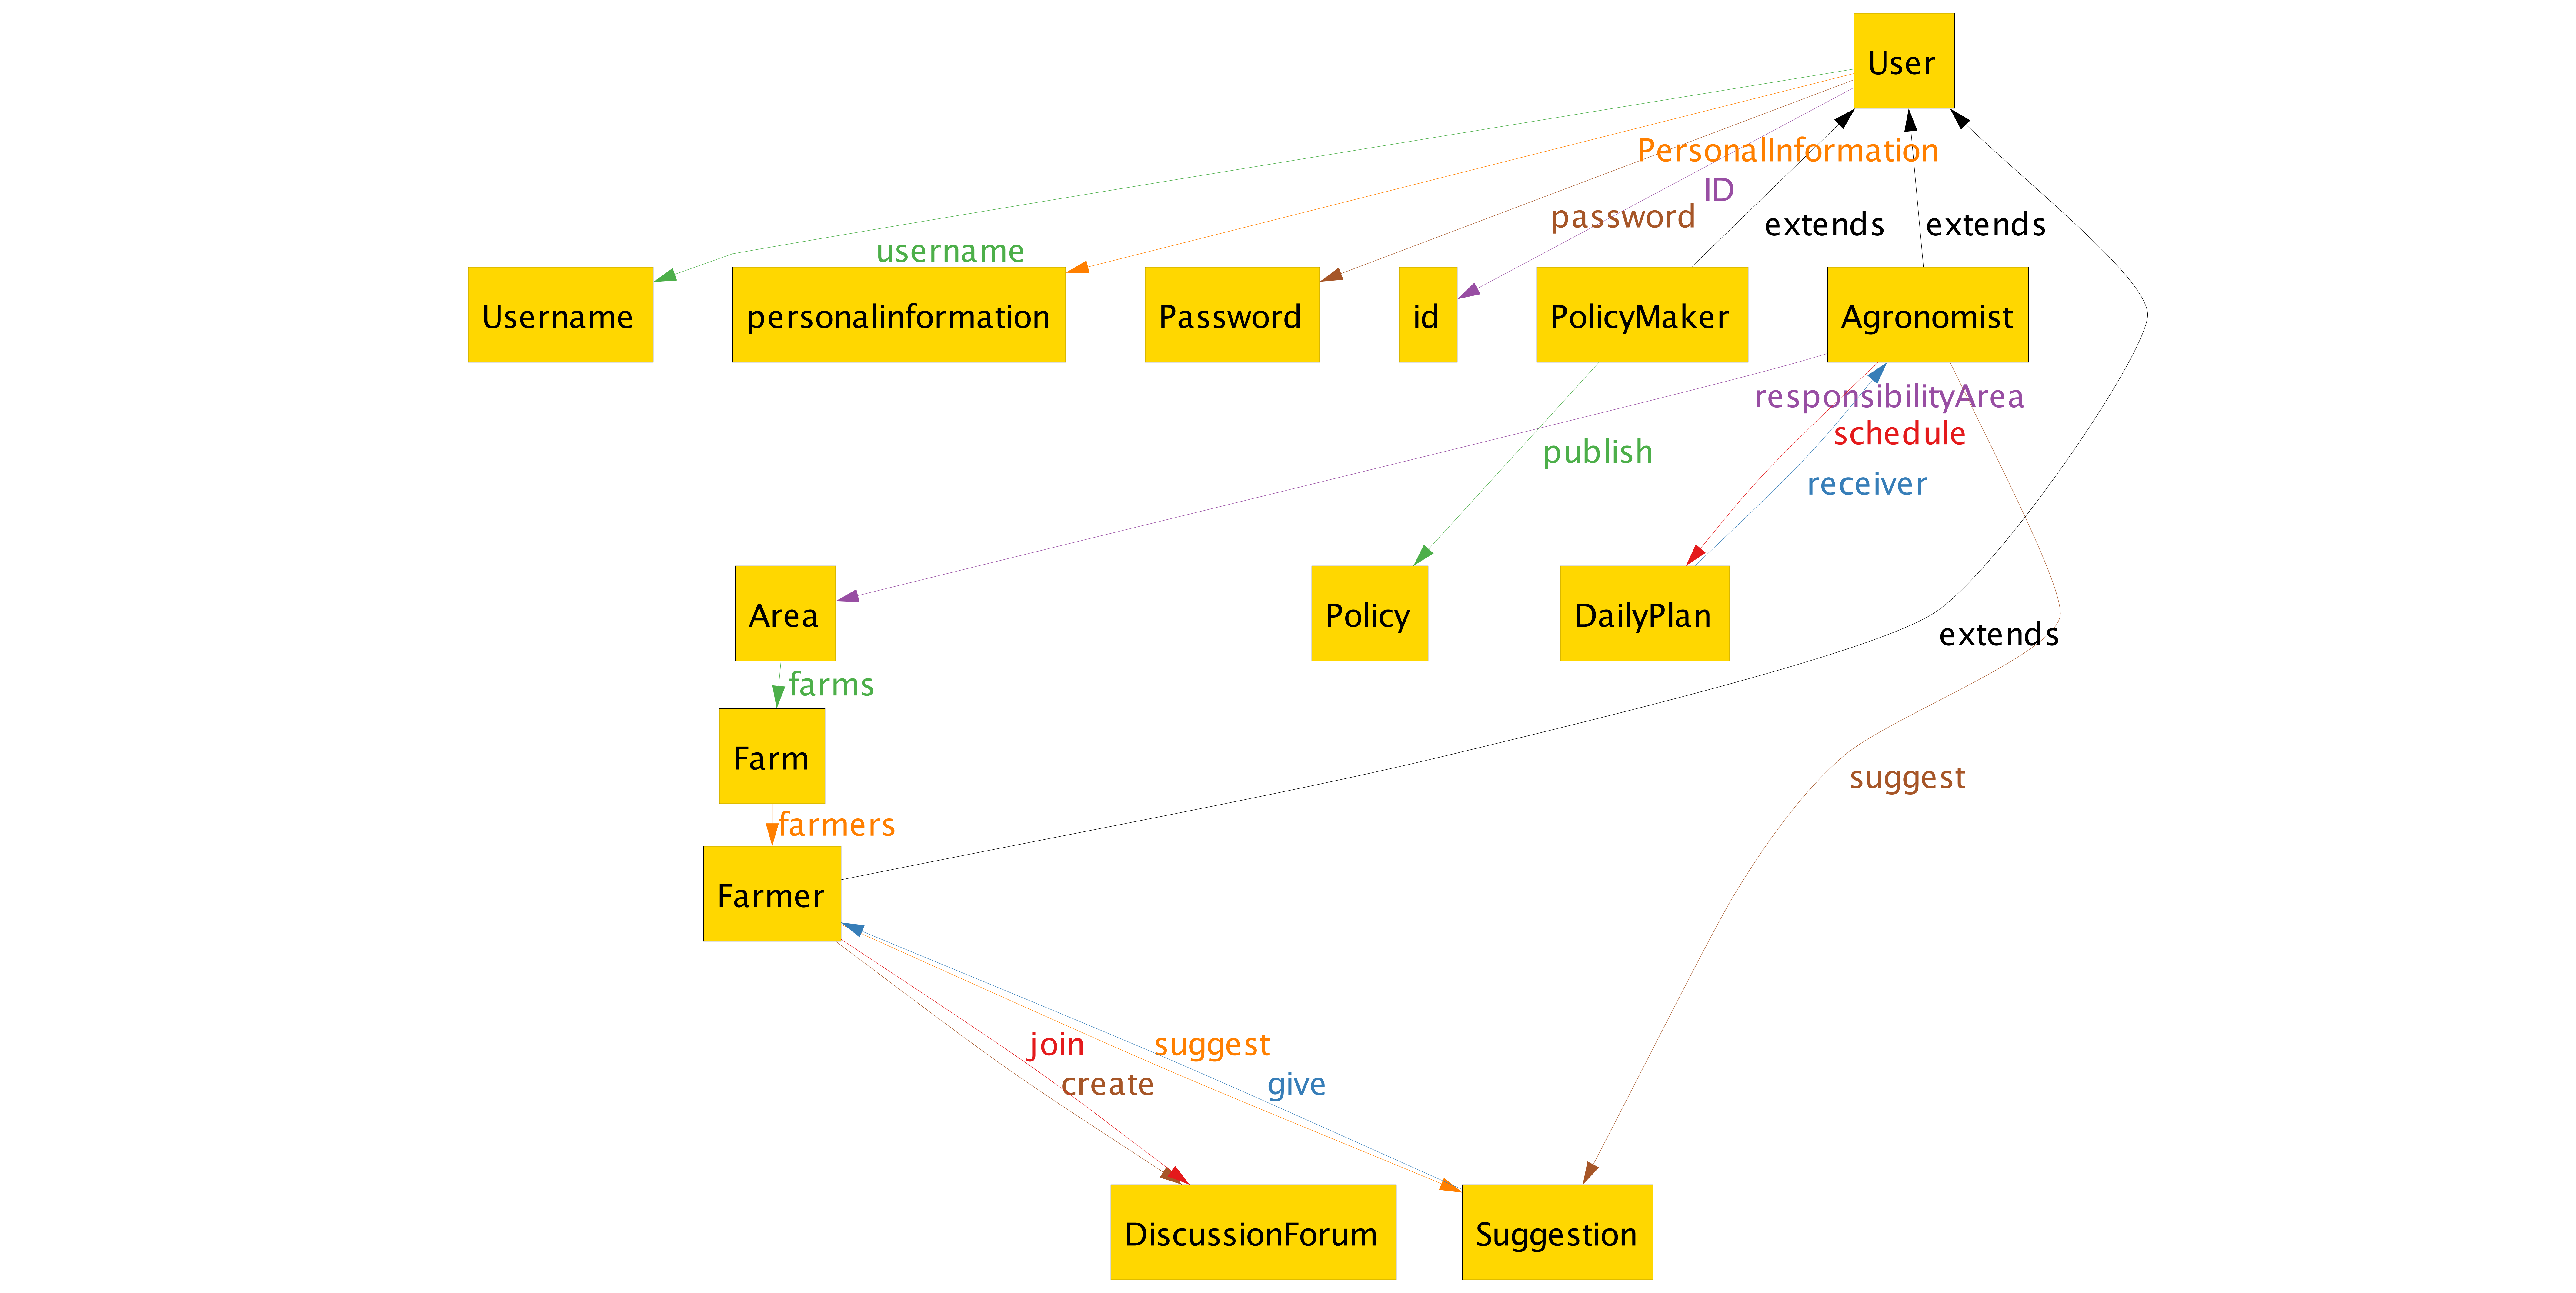
\includegraphics[width=\textwidth]{RASD/image/Alloy2.png}
  \caption{One of the worlds generated}
\end{figure}

\begin{figure}[H]
  \centering
  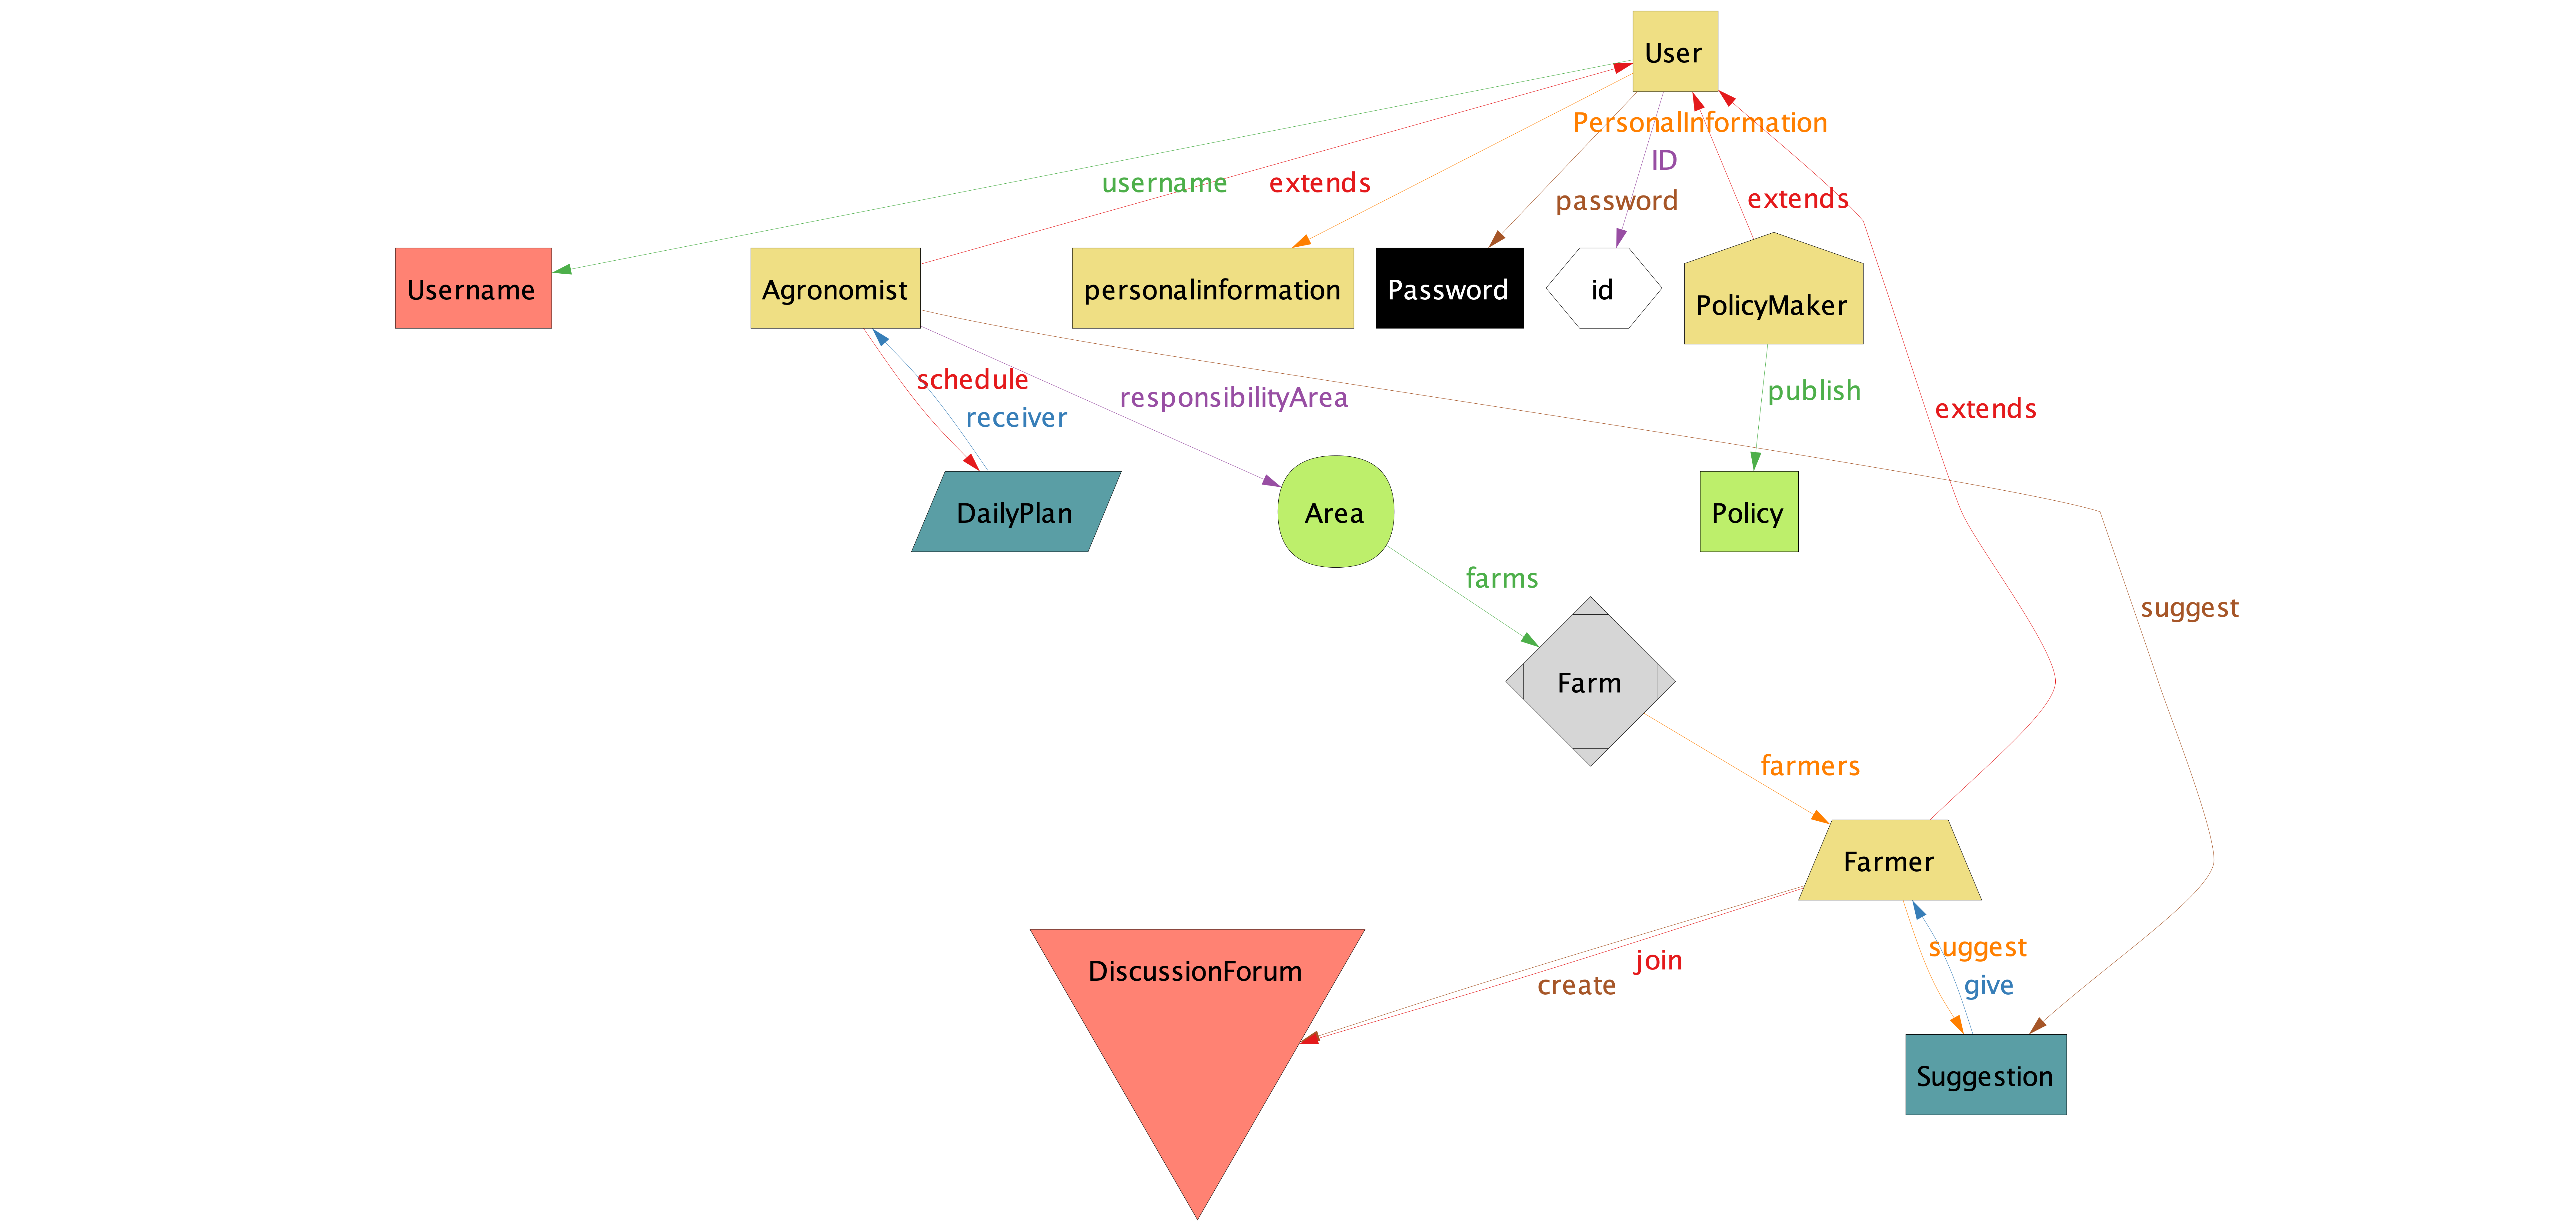
\includegraphics[width=\textwidth]{RASD/image/Alloy3.png}
  \caption{One of the worlds generated}
\end{figure}


\end{document}
